%PDF DI RIFERIMENTO: 03_Requirement Engineering.pdf

\chapter{Requirement Analysis}
    \section{Obiettivo}
        In questa sezione verranno analizzate le informazioni definite nei requisiti di sistema al fine di schematizzare opportunamente il dominio del problema.

    \section{Use Case Diagram}
        %Use Case Diagram costruito con StarUML
        \begin{figure}[htbp!]
            \centering
                \vspace{2\baselineskip}
                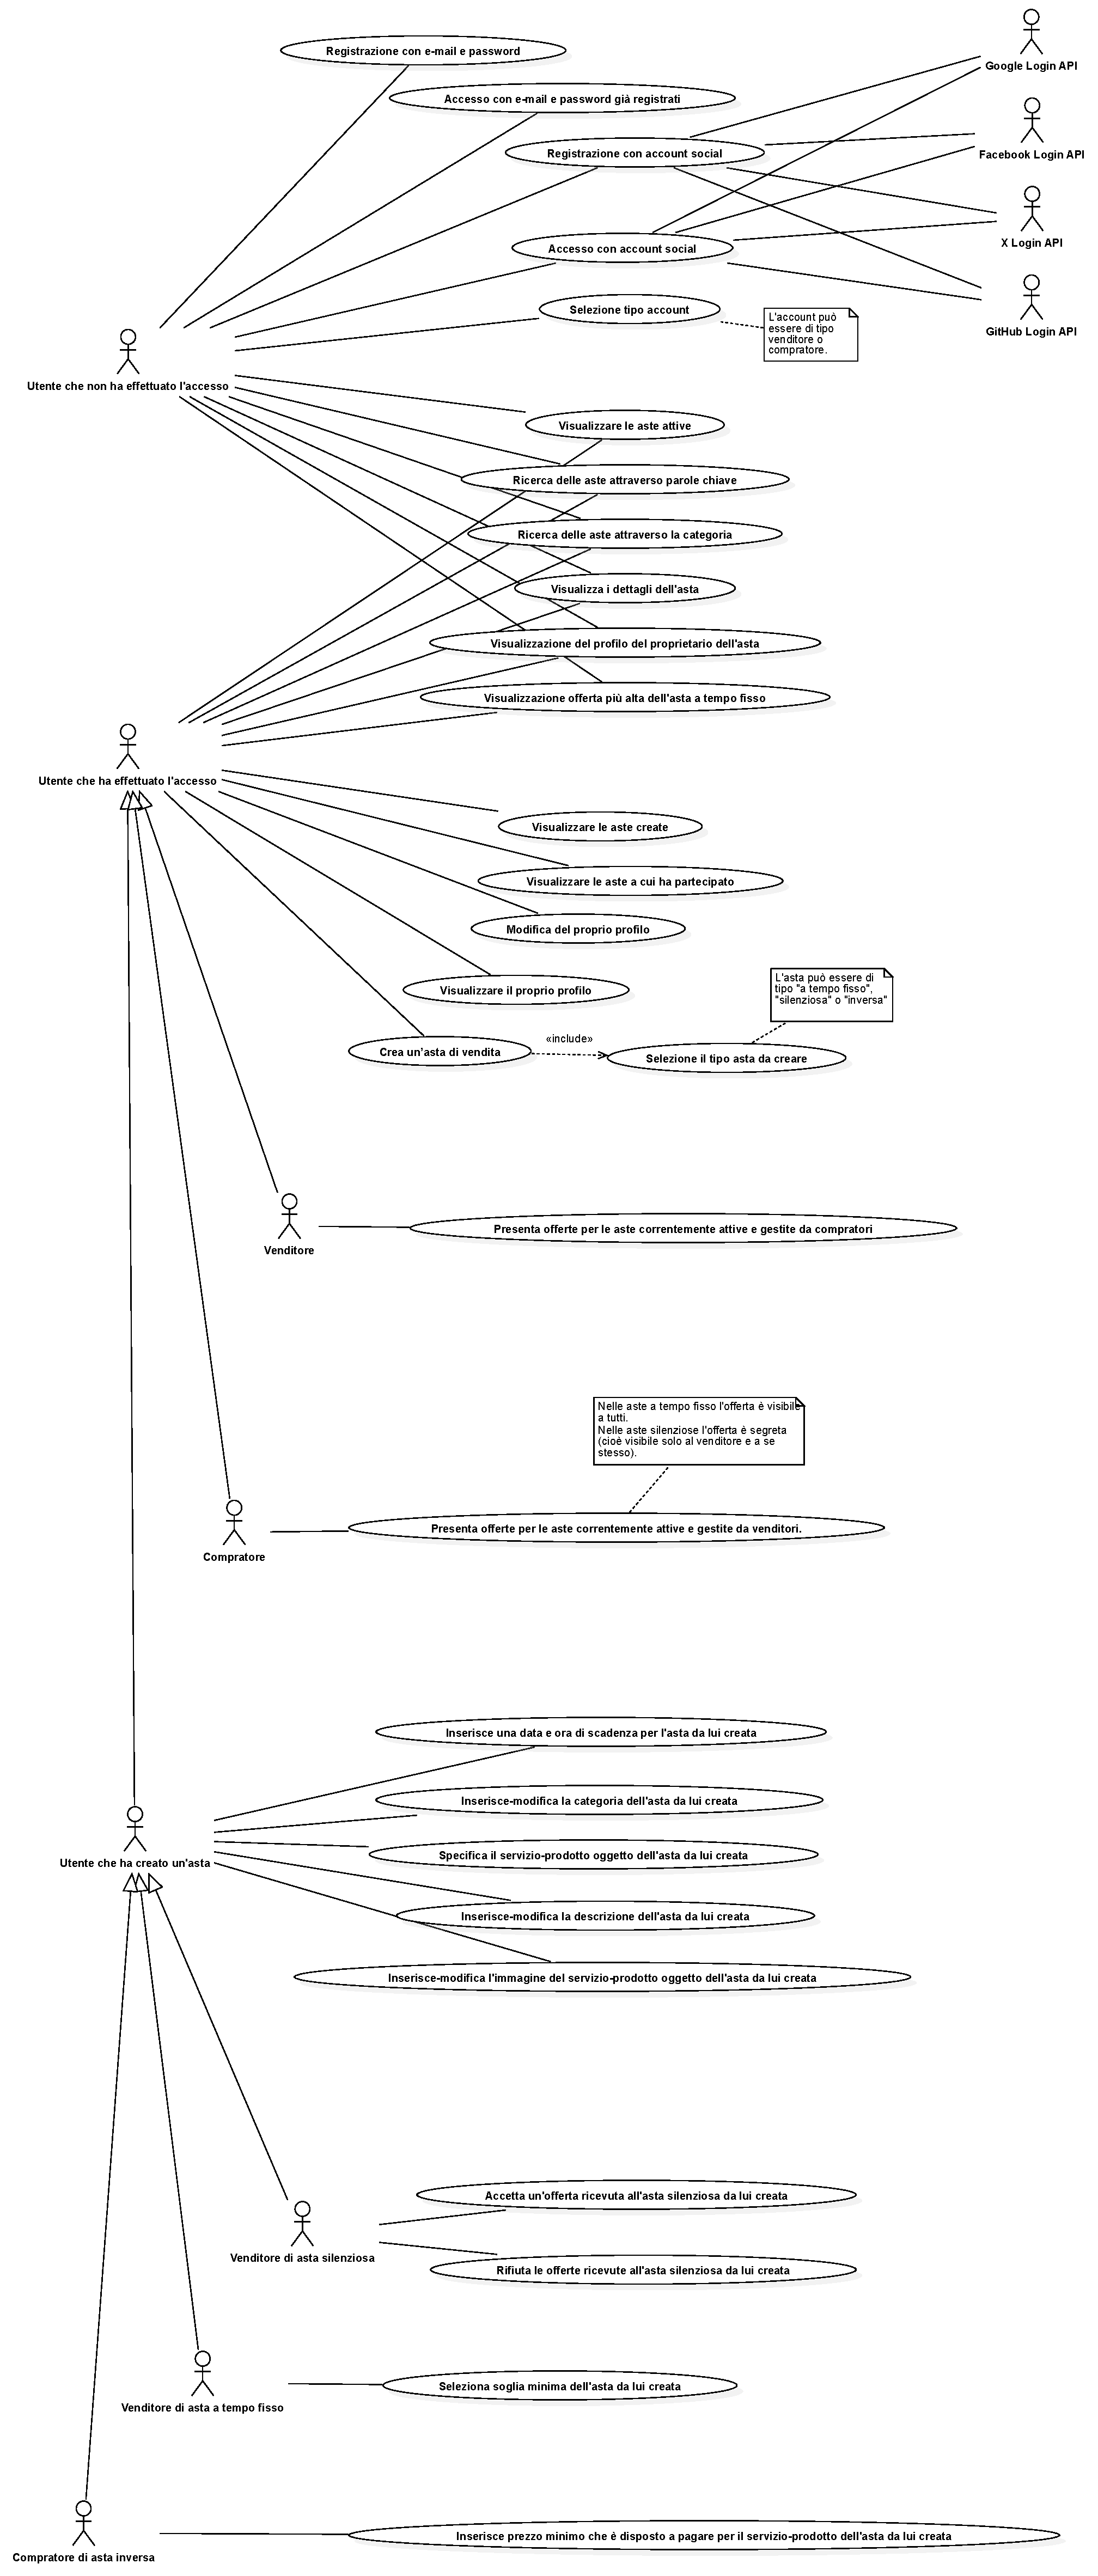
\includegraphics[width=0.41\linewidth]{Immagini/Diagrammi/UseCaseDiagram.pdf}
            \caption{Use Case Diagram}
            \label{fig:Use Case Diagram}
        \end{figure}

    \newpage
    
    \section{Target utenti}
        La personas principale scelta è Maria Lombardo. La personas secondaria è Luca Serra
        
        \begin{figure}[!htb]
           \begin{minipage}{0.48\textwidth}
                \centering
             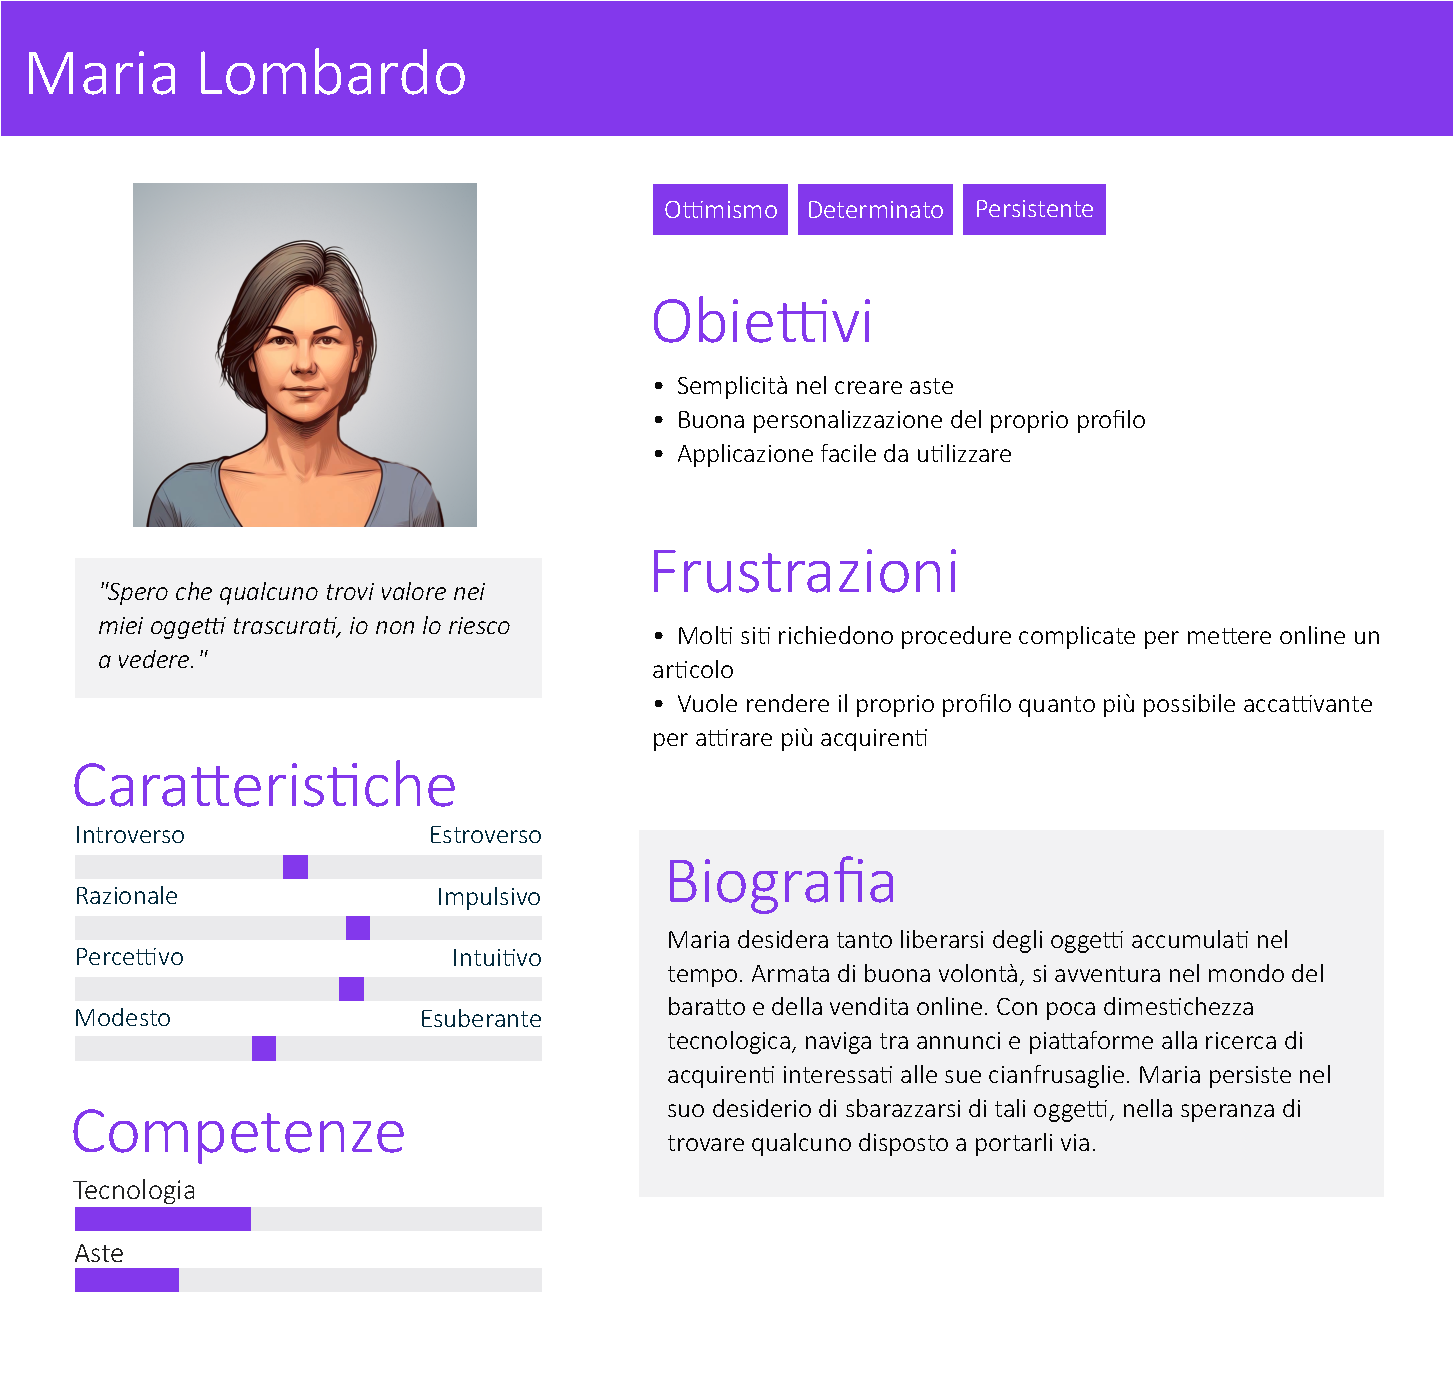
\includegraphics[width=.7\linewidth]{Immagini/Personas/Maria Lombardo.pdf}
             \caption{Maria Lombardo}\label{Fig:Maria Lombardo}
           \end{minipage}\hfill
           \begin{minipage}{0.48\textwidth}
                \centering
             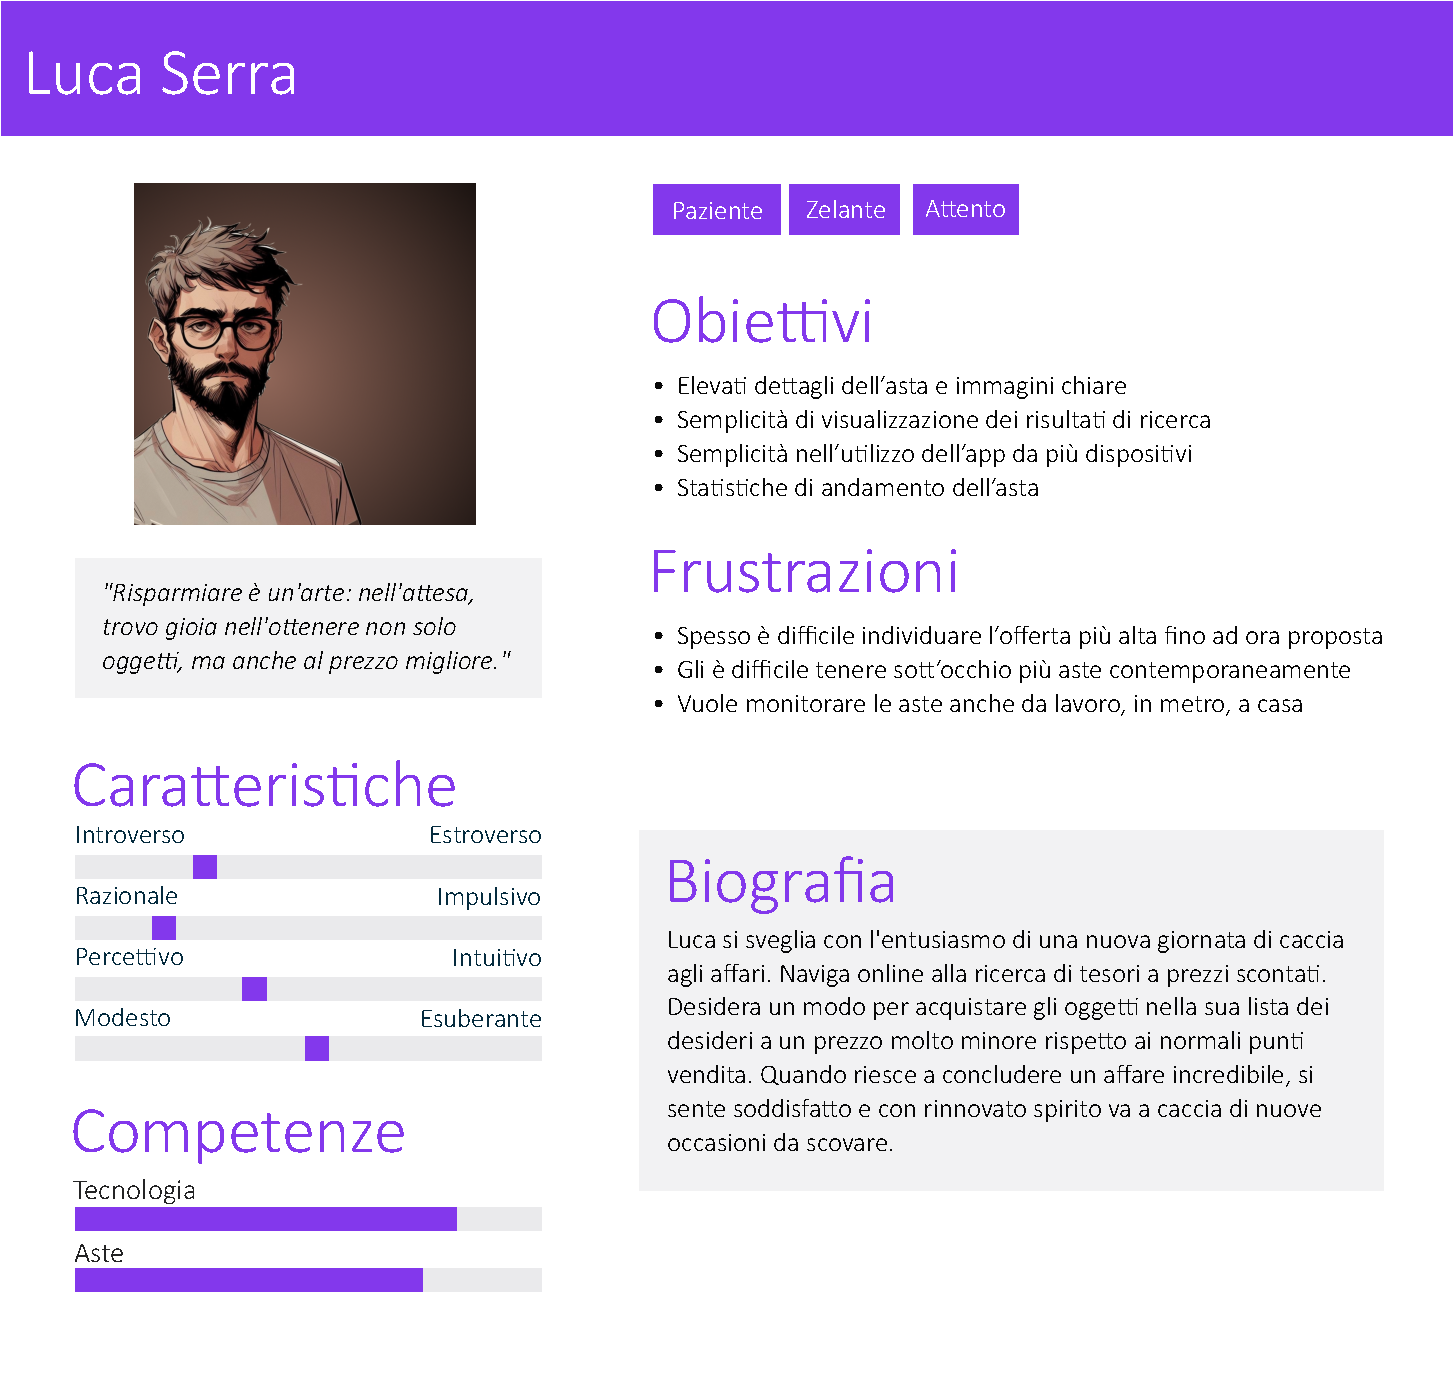
\includegraphics[width=.7\linewidth]{Immagini/Personas/Luca Serra.pdf}
             \caption{Luca Serra}\label{Fig:Luca Serra}
           \end{minipage}
        \end{figure}

        \begin{figure}[!htb]
           \begin{minipage}{0.48\textwidth}
                \centering
             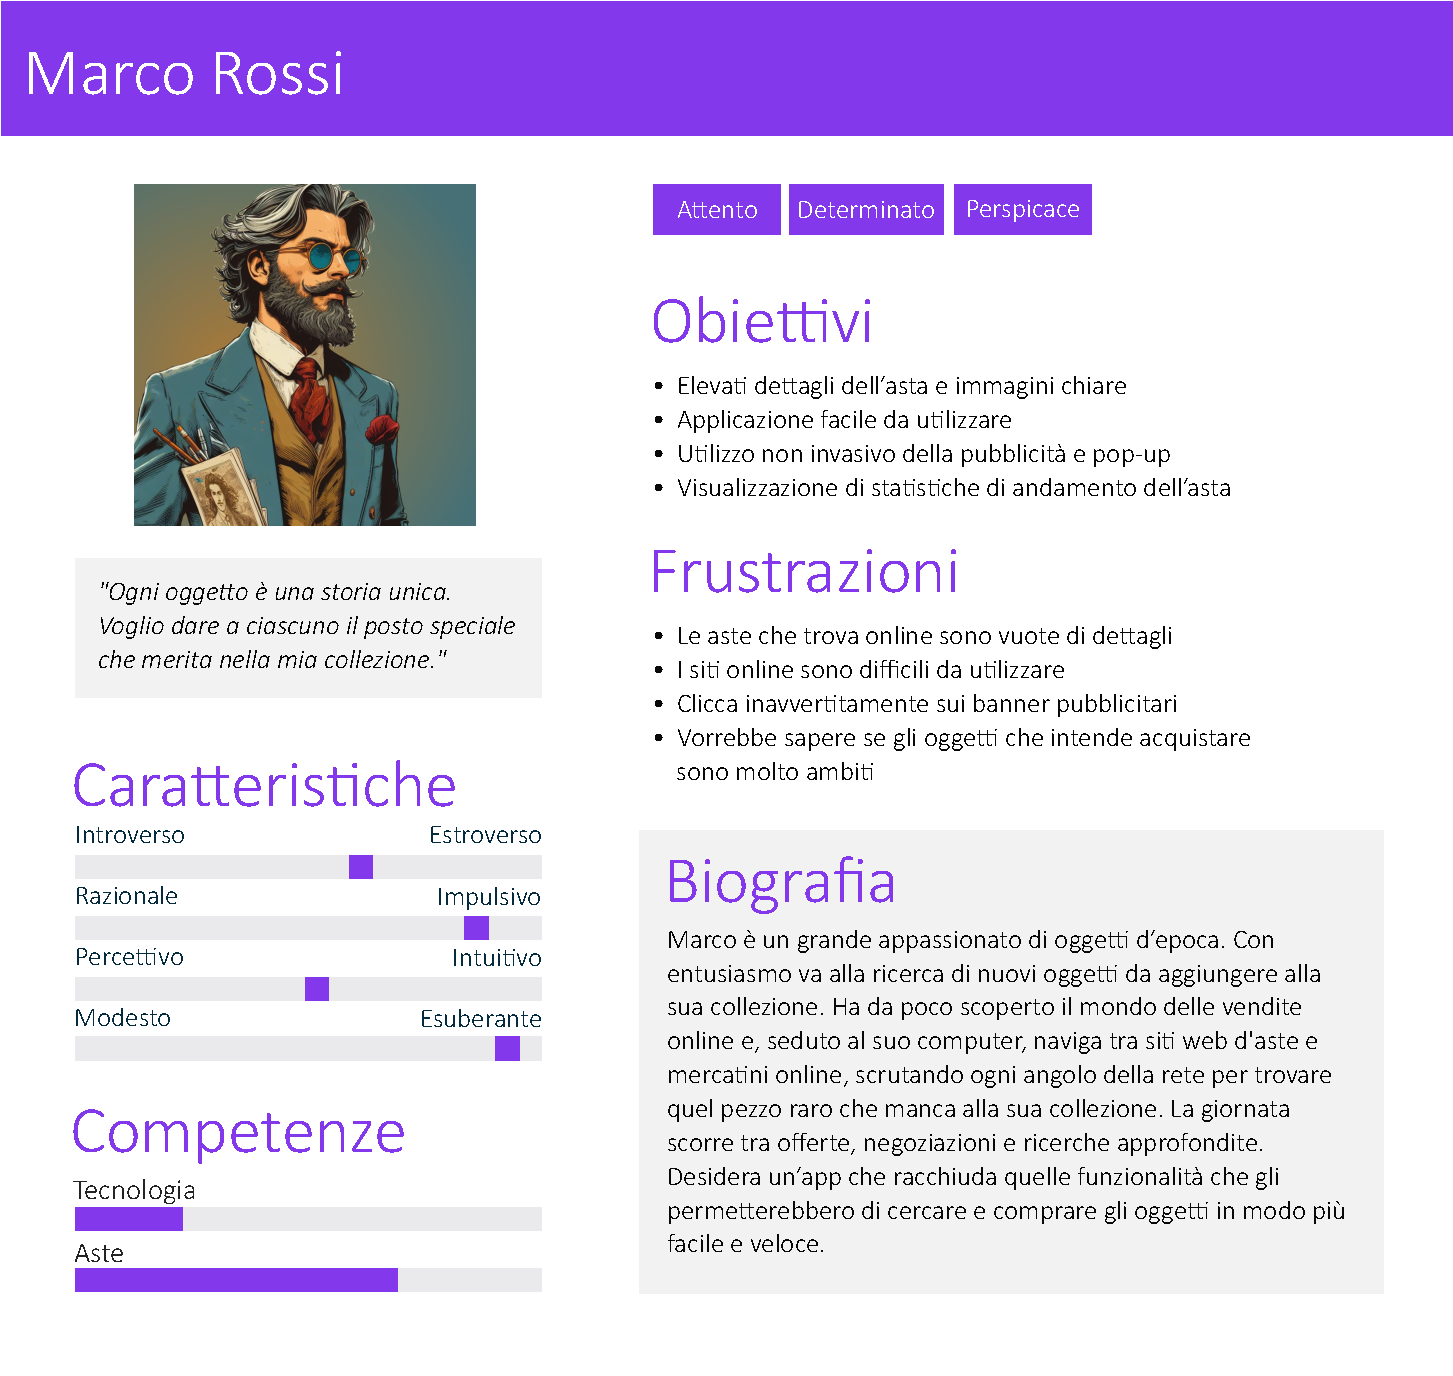
\includegraphics[width=.7\linewidth]{Immagini/Personas/Marco Rossi.pdf}
             \caption{Marco Rossi}\label{Fig:Marco Rossi}
           \end{minipage}\hfill
           \begin{minipage}{0.48\textwidth}
                \centering
             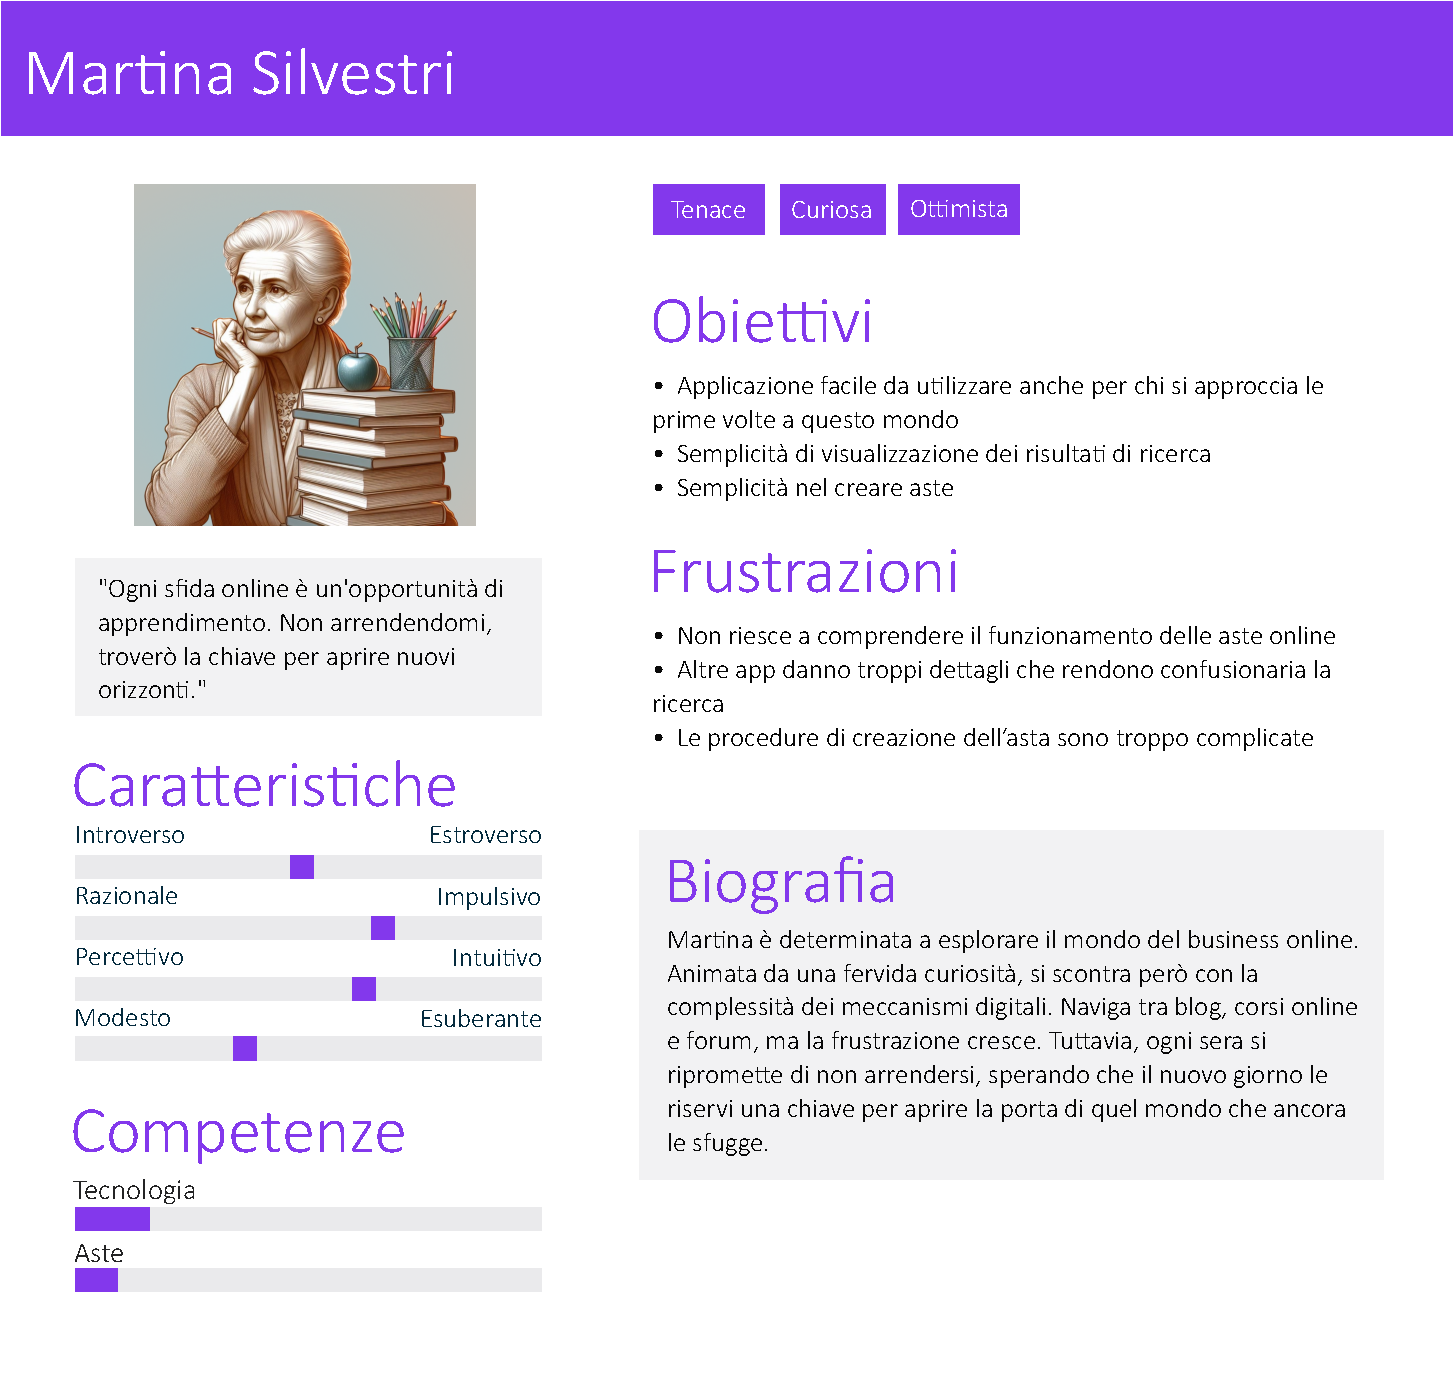
\includegraphics[width=.7\linewidth]{Immagini/Personas/Martina Silvestri.pdf}
             \caption{Martina Silvestri}\label{Fig:Martina Silvestri}
           \end{minipage}
        \end{figure}

        \begin{figure}[!htb]
           \begin{minipage}{0.48\textwidth}
                \centering
             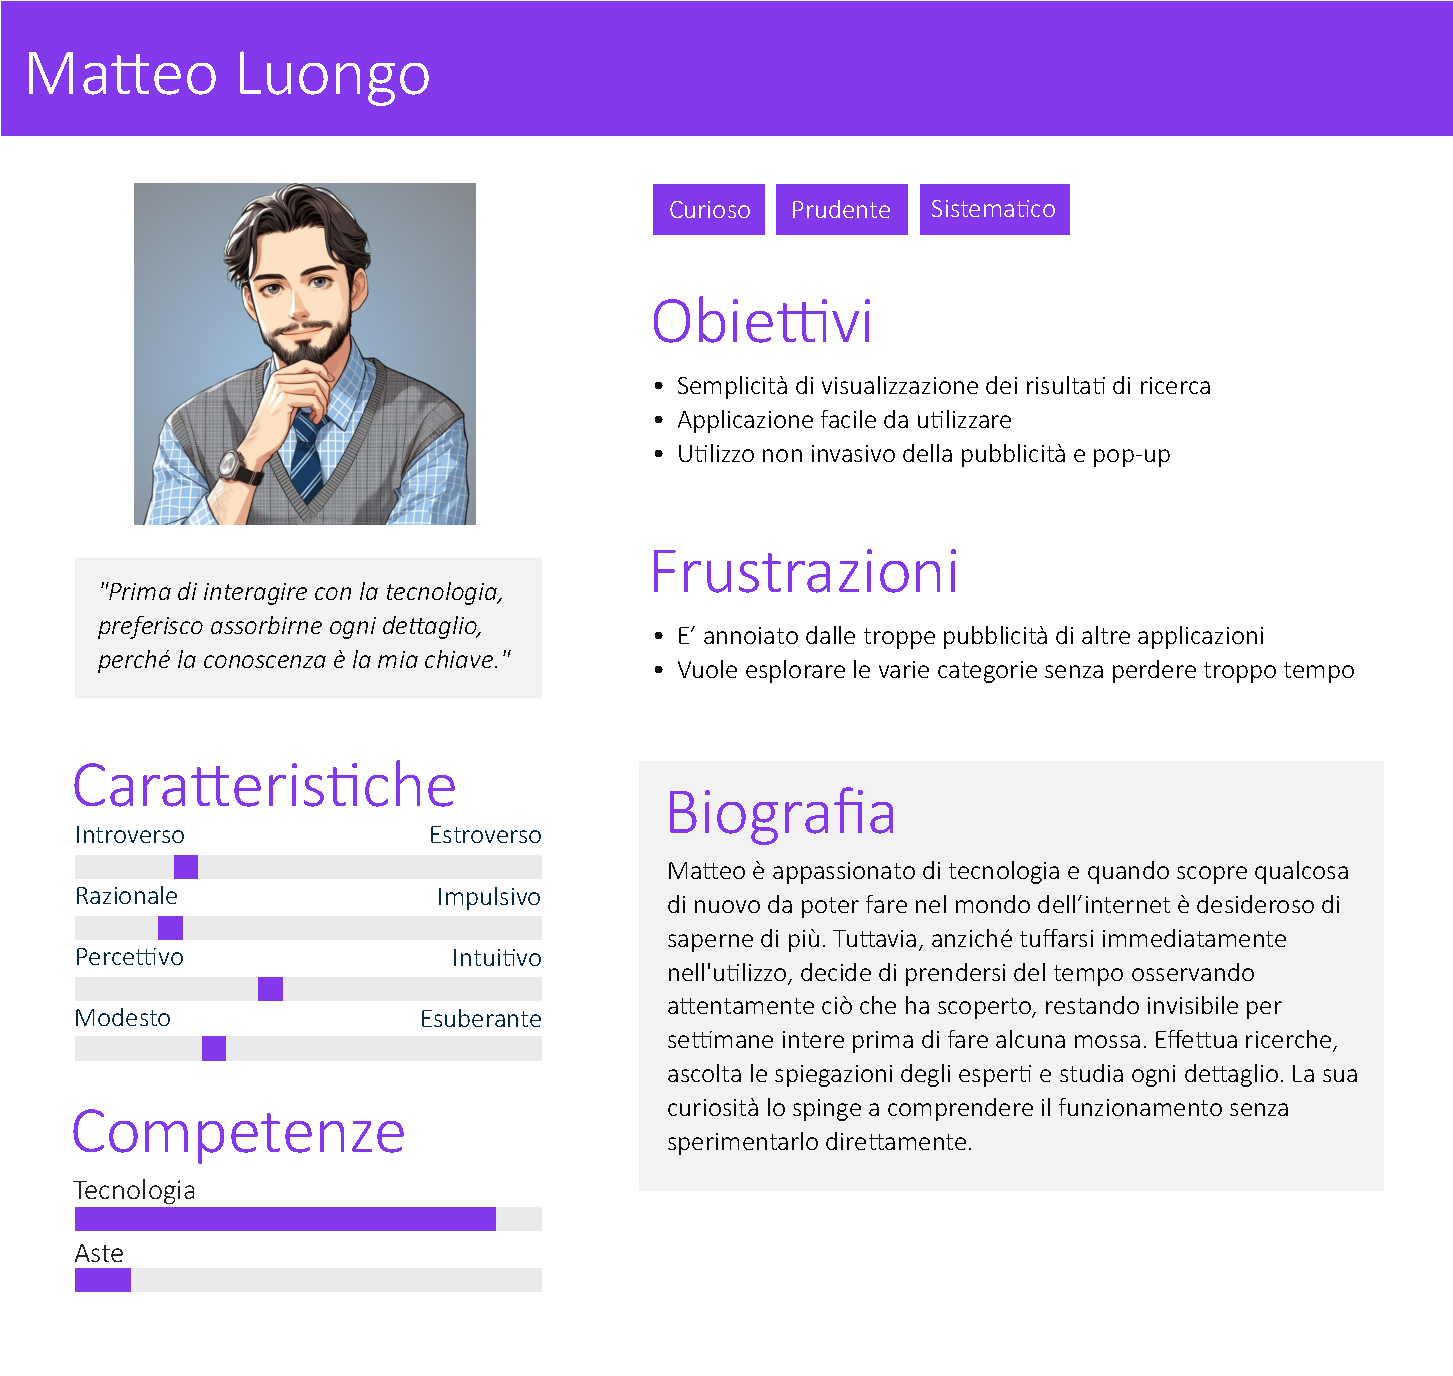
\includegraphics[width=.7\linewidth]{Immagini/Personas/Matteo Luongo.pdf}
             \caption{Matteo Luongo}\label{Fig:Matteo Luongo}
           \end{minipage}\hfill
           \begin{minipage}{0.48\textwidth}
                \centering
             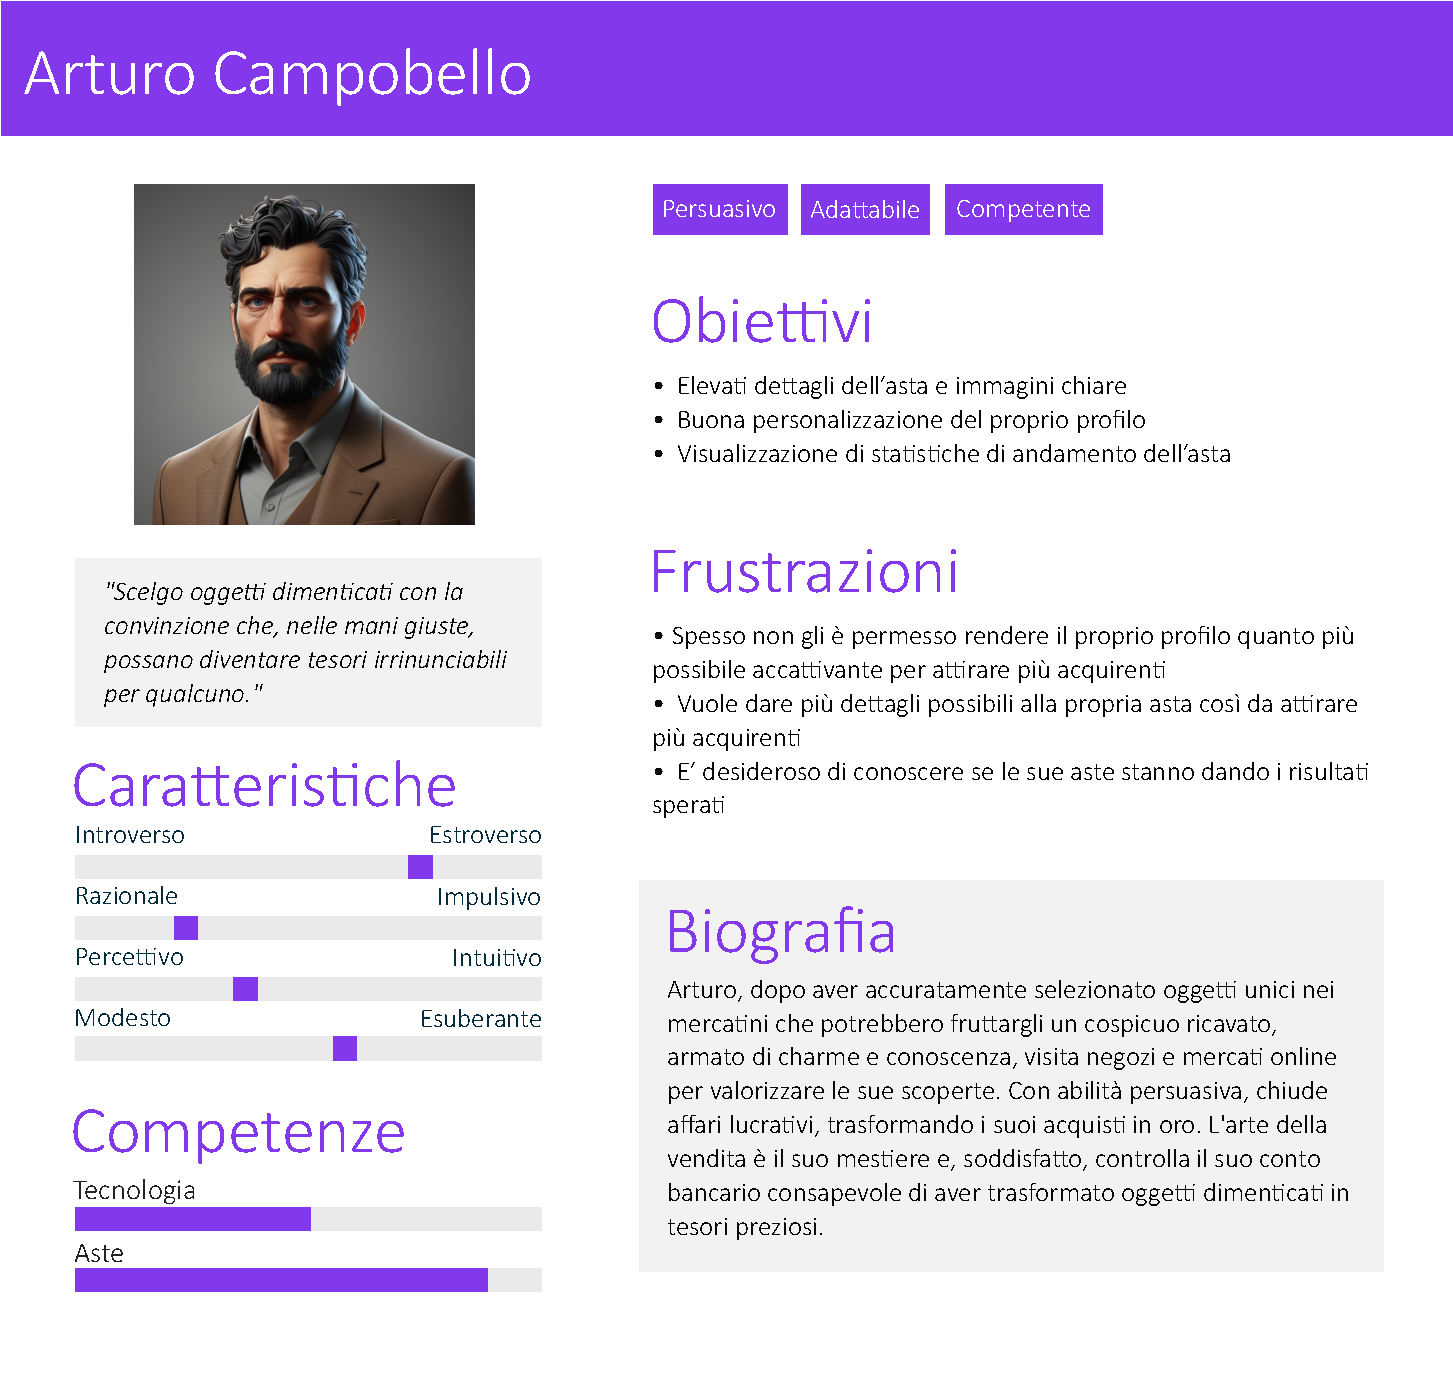
\includegraphics[width=.7\linewidth]{Immagini/Personas/Arturo Campobello.pdf}
             \caption{Arturo Campobello}\label{Fig:Arturo Campobello}
           \end{minipage}
        \end{figure}
        
    \section{Mockup}

    \newpage

    \section{Tabelle di Cockburn}
        \subsection{Crea un’asta inversa}
            \begin{longtable}{|C{3.0cm}|C{1.3cm}|L{5.2cm}|L{5.2cm}|}
                \hline
                    \textbf{USE CASE \#1} &
                    \multicolumn{3}{|l|}{\textbf{Crea un’asta inversa}}\\
                \hline
                    Goal in Context &
                    \multicolumn{3}{|l|}{L'utente di tipo "compratore" vuole creare un'asta inversa.}\\
                \hline
                    Preconditions &
                    \multicolumn{3}{|l|}{L'utente ha effettuato l'accesso con un account di tipo "compratore".}\\
                \hline
                    Success End Condition &
                    \multicolumn{3}{|l|}{L'utente di tipo "compratore" ha correttamente creato un'asta "inversa"}\\
                \hline
                    \multirow[|c|]{30}{*}{DESCRIPTION} 
                    & \textbf{Step n°}
                    & \textbf{Compratore}
                    & \textbf{Sistema}\\
                \cline{2-4}
                        & 1
                        & Preme bottone "Crea asta" su Mockup C1
                        & \\
                \cline{2-4}
                        & 2
                        & 
                        & Mostra Mockup C4 con tutte le informazioni dell'asta da poter inserire.\\
                \cline{2-4}
                        & 3
                        & Preme sul campo di input "Data di scadenza"
                        & \\
                \cline{2-4}
                        & 4
                        & 
                        & Mostra il pannello di selezione della data da calendario\\
                \cline{2-4}
                        & 5
                        & Seleziona la data
                        & \\
                \cline{2-4}
                        & 6
                        & Clicca su OK
                        & \\
                \cline{2-4}
                        & 7
                        & 
                        & Scrive la data selezionata nel campo di input "Data di scadenza"\\
                \cline{2-4}
                        & 8
                        & Preme sul campo di input "Ora di scadenza"
                        & \\
                \cline{2-4}
                        & 9
                        & 
                        & Mostra il pannello di selezione dell'ora\\
                \cline{2-4}
                        & 10
                        & Seleziona l'ora
                        & \\
                \cline{2-4}
                        & 11
                        & Clicca su OK
                        & \\
                \cline{2-4}
                        & 12
                        & 
                        & Scrive l'ora selezionata nel campo di input "Ora di scadenza"\\
                \cline{2-4}
                        & 13
                        & Preme sul campo di input "Prezzo di partenza"
                        & \\
                \cline{2-4}
                        & 14
                        &
                        & Mostra il tastierino numerico \\
                \cline{2-4}
                        & 15
                        & Inserisce il prezzo di partenza
                        & \\
                \cline{2-4}
                        & 16
                        & Preme sul campo di input "Nome prodotto"
                        & \\
                \cline{2-4}
                        & 17
                        &
                        & Mostra la tastiera \\
                \cline{2-4}
                        & 18
                        & Inserisce il nome del prodotto oggetto dell'asta
                        & \\
                \cline{2-4}
                        & 19
                        & Preme sul campo di input "Categoria"
                        & \\
                \cline{2-4}
                        & 20
                        &
                        & Mostra il menù a tendina con le diverse categorie tra cui scegliere \\
                \cline{2-4}
                        & 21
                        & Seleziona la categoria
                        & \\
                \cline{2-4}
                        & 22
                        & 
                        & Scrive la categoria scelta nel campo di input "Categoria"\\
                \cline{2-4}
                        & 23
                        & Preme sul campo di input "Descrizione"
                        & \\
                \cline{2-4}
                        & 24
                        &
                        & Mostra la tastiera \\
                \cline{2-4}
                        & 25
                        & Inserisce la descrizione del prodotto oggetto dell'asta
                        & \\
                \cline{2-4}
                        & 26
                        & Preme sul pulsante "Crea"
                        & \\
                \cline{2-4}
                        & 27
                        & 
                        & Mostra Mockup P20 (Pop-up di successo)\\
                \cline{2-4}
                        & 28
                        & Preme il pulsante X sul Mockup P20
                        & \\
                \cline{2-4}
                        & 29
                        & 
                        & Torna al Mockup C1 (Home)\\
                \hline
                    EXTENSIONS
                    & \textbf{Step n°} 
                    & \textbf{Compratore} 
                    & \textbf{Sistema}\\
                \hline
                    \multirow[|c|]{3}{*}{\shortstack[c]{Seleziona data \\  antecedente a \\quella odierna}}
                        & 7.a
                        & 
                        & Mostra Mockup P19 con testo "Non puoi inserire una data antecedente a quella odierna!"\\
                \cline{2-4}
                        & 8.a
                        & Clicca su X sul Mockup P19
                        & \\
                \cline{2-4}
                        & 9.a
                        & 
                        & Continua da step 3 di main scenario\\
                \hline
                    \multirow[|c|]{3}{*}{\shortstack[c]{Seleziona data \\ odierna e ora \\ antecedente a \\quella attuale}}
                        & 12.a
                        & 
                        & Mostra Mockup P14 con testo "Non puoi selezionare un’ora antecedente a quella attuale in data odierna!"\\
                \cline{2-4}
                        & 13.a
                        & Clicca su X sul Mockup P14
                        & \\
                \cline{2-4}
                        & 14.a
                        & 
                        & Continua da step 8 di main scenario\\
                \hline
                    \multirow[|c|]{3}{*}{\shortstack[c]{Seleziona prezzo di \\ partenza negativo}}
                        & 16.b
                        & 
                        & Mostra Mockup P10 con testo "Non puoi inserire una somma di partenza minore di 0 €."\\
                \cline{2-4}
                        & 17.b
                        & Clicca su X sul Mockup P10
                        & \\
                \cline{2-4}
                        & 16.b
                        & 
                        & Continua da step 13 di main scenario\\
                \hline
                    \multirow[|c|]{2}{*}{\shortstack[c]{Alcuni campi \\ obbligatori non \\ compilati}}
                        & 27.c
                        & 
                        & Mostra Mockup E11 dove vengono segnalati in rosso i campi obbligatori non compilati\\
                \cline{2-4}
                        & 28.c
                        & Riparte da step 3 di main scenario, saltando i campi di input già compilati
                        & \\
                \hline
                    \multirow[|c|]{4}{*}{\shortstack[c]{Esce dalla pagina \\ di creazione asta}}
                        & \textit{In qualunque passo del main scenario}
                        & Preme qualsiasi tasto di navigazione (della navbar in basso o tasto "indietro" del dispositivo)
                        & \\
                \cline{2-4}
                        & 
                        & 
                        & Mostra Mockup P6 con testo "Se uscirai da questa schermata, i dati inseriti nei campi saranno cancellati. Vuoi proseguire?" \\
                \cline{2-4}
                        & 
                        & Clicca su Esci sul Mockup P6
                        & \\
                \cline{2-4}
                        & 
                        & 
                        & Mostra Mockup corrispondente al tasto cliccato\\
                \hline
                    SUBVARIATIONS
                    & \textbf{Step n°} 
                    & \textbf{Compratore} 
                    & \textbf{Sistema}\\
                \hline
                    \multirow[|c|]{1}{*}{\shortstack[c]{Inserisce immagine}}
                        & 16.s1
                        & Preme sul campo di input "Aggiungi immagine prodotto"
                        & \\
                \cline{2-4}
                        & 17.s1
                        & 
                        & Mostra il sistema per selezionare le immagini\\
                \cline{2-4}
                        & 18.s1
                        & Seleziona una o più immagini
                        & \\
                \cline{2-4}
                        & 19.s1
                        & Clicca su OK
                        & \\
                \cline{2-4}
                        & 20.s1
                        & 
                        & Continua da step 16 di main scenario\\
                \hline
            \end{longtable}

        \newpage

        \subsection{Accetta un'offerta ricevuta all'asta silenziosa}
            \begin{longtable}{|C{3.0cm}|C{1.3cm}|L{5.2cm}|L{5.2cm}|}
                \hline
                    \textbf{USE CASE \#2} &
                    \multicolumn{3}{|l|}{\textbf{Accetta un'offerta ricevuta all'asta silenziosa}}\\
                \hline
                    Goal in Context &
                    \multicolumn{3}{|l|}{\shortstack[l]{L'utente di tipo "venditore" vuole accettare un'offerta ricevuta in un'asta \\ "silenziosa" da lui creata}}\\
                \hline
                    Preconditions &
                    \multicolumn{3}{|l|}{\shortstack[l]{L'utente ha effettuato l'accesso con un account di tipo "venditore" e ha creato \\ un'asta "silenziosa"}}\\
                \hline
                    Success End Condition &
                    \multicolumn{3}{|l|}{\shortstack[l]{L'utente di tipo "venditore" ha correttamente accettato un'offerta di un'asta \\ "silenziosa" da lui creata}}\\
                \hline
                    \multirow[|c|]{11}{*}{DESCRIPTION} 
                    & \textbf{Step n°}
                    & \textbf{Venditore di asta silenziosa}
                    & \textbf{Sistema}\\
                \cline{2-4}
                        & 1
                        & Preme bottone "Profilo" su Mockup V1
                        & \\
                \cline{2-4}
                        & 2
                        & 
                        & Mostra Mockup V7 con tutte le opzioni per utenti loggati.\\
                \cline{2-4}
                        & 3
                        & Preme sul bottone "Le mie aste create".
                        & \\
                \cline{2-4}
                        & 4
                        & 
                        & Mostra il Mockup V11 con tutte le aste create dal venditore.\\
                \cline{2-4}
                        & 5
                        & Clicca sull'icona a forma di elenco dell'asta di cui si vogliono visualizzare le offerte ricevute.
                        & \\
                \cline{2-4}
                        & 6
                        & 
                        & Mostra Mockup V13 con l'elenco di tutte le offerte ricevute.\\
                \cline{2-4}
                        & 7
                        & Clicca sulla spunta verde dell'offerta che si vuole accettare.
                        & \\
                \cline{2-4}
                        & 8
                        & 
                        & Mostra il Mockup P7 con testo "Confermi di voler accettare questa offerta? Tutte le altre saranno automaticamente rifiutate."\\
                \cline{2-4}
                        & 9
                        & Clicca sul pulsante "Accetta"
                        & \\
                \cline{2-4}
                        & 10
                        & 
                        & Mostra Mockup V14 dove vengono elencate tutte le offerte ricevute a questa asta "silenziosa". L'offerta accettata sarà l'unica in bianco, tutte le altre saranno in grigio.\\
                \hline
                    EXTENSIONS
                    & \textbf{Step n°} 
                    & \textbf{Venditore di asta silenziosa} 
                    & \textbf{Sistema}\\
                \hline
                    \multirow[|c|]{2}{*}{\shortstack[c]{Esce dalla pagina \\ di gestione delle \\ offerta ricevute}}
                        & 7.a
                        & Preme sul tasto "indietro" (del dispositivo o dell'interfaccia)
                        & \\
                \cline{2-4}
                        & 8.a
                        & 
                        & Mostra Mockup nel quale ci si trovava in precedenza\\
                \hline
                    SUBVARIATIONS
                    & \textbf{Step n°} 
                    & \textbf{Venditore di asta silenziosa}
                    & \textbf{Sistema}\\
                \hline
                    \multirow[|c|]{4}{*}{\shortstack[c]{Riceve notifica \\ di proposta offerta \\ per l'asta silenziosa}}
                        & 1.s1
                        & Preme sul bottone "Notifiche"
                        & \\
                \cline{2-4}
                        & 2.s1
                        & 
                        & Mostra il Mockup V6 con la notifica relativa all'offerta ricevuta\\
                \cline{2-4}
                        & 3.s1
                        & Clicca sulla notifica
                        & \\
                \cline{2-4}
                        & 4.s1
                        &
                        & Continua con step 6 di main scenario\\
                \hline
            \end{longtable}

    \newpage

    \section{Valutazione dell’usabilità a priori}
        \subsection{Valutazioni con utenti}
            Sono stati effettuati una serie di valutazioni di usabilità attraverso i prototipi costruiti con strumenti di rapid prototyping, in particolare “Figma”. In particolare, nelle tabelle seguenti sono riportati tutti i casi d'uso testati e, per ogni utente, viene indicato con:
            \begin{itemize}
                \item S = Successo (ovvero la task è stata completata velocemente e senza intoppi)
                \item P = Successo parziale (ovvero è stato necessario un po' di tempo in più e piccoli suggerimenti)
                \item F = Fallimento (ovvero la task non è stata completata nonostante i piccoli suggerimenti)
                \item X = Non testato
            \end{itemize}
        
            \begin{table}[ht]
            \resizebox{\textwidth}{!}{
                \begin{tabular}{l|l|l|l|l|l|l|l|l|l|}
                \cline{2-10}
                &
                \begin{tabular}[c]{@{}l@{}}Registrazione\\ account\end{tabular} &
                \begin{tabular}[c]{@{}l@{}}Accesso\\ account\end{tabular} &
                \begin{tabular}[c]{@{}l@{}}Ricerca\\ aste\end{tabular} &
                \begin{tabular}[c]{@{}l@{}}Filtra\\ aste\end{tabular} &
                \begin{tabular}[c]{@{}l@{}}Visualizza\\ dettagli asta\end{tabular} &
                \begin{tabular}[c]{@{}l@{}}Visualizza\\ profilo\\ proprietario\\ asta\end{tabular} &
                \begin{tabular}[c]{@{}l@{}}Visualizza\\ le tue aste\\ create\end{tabular} &
                \begin{tabular}[c]{@{}l@{}}Modifica\\ la tua\\ asta\end{tabular} &
                \begin{tabular}[c]{@{}l@{}}Elimina\\ la tua\\ asta\end{tabular}\\ \hline
                \multicolumn{1}{|l|}{Utente 1} & S & S & S & S & S & S & S & S & S \\ \hline
                \multicolumn{1}{|l|}{Utente 2} & S & S & S & P & S & P & S & S & S \\ \hline
                \multicolumn{1}{|l|}{Utente 3} & S & S & S & S & S & S & S & S & S \\ \hline
                \multicolumn{1}{|l|}{Utente 4} & S & S & S & S & S & P & S & S & S \\ \hline
                \multicolumn{1}{|l|}{Utente 5} & S & S & S & S & P & P & P & S & S \\ \hline
                \multicolumn{1}{|l|}{Utente 6} & S & S & S & S & P & S & P & S & S \\ \hline %Kevin
                \multicolumn{1}{|l|}{Utente 7} & S & S & X & X & P & P & S & S & S \\ \hline %Nancy
                \multicolumn{1}{|l|}{Utente 8} & S & S & S & S & S & S & P & S & S \\ \hline %Cristina
                \multicolumn{1}{|l|}{Utente 9} & S & S & X & X & S & S & S & P & S \\ \hline %Francesco
                \end{tabular}
                }
            \end{table}
    
            \begin{table}[ht]
            \resizebox{\textwidth}{!}{
                \begin{tabular}{l|l|l|l|l|l|l|l|l|}
                \cline{2-9}
                &
                \begin{tabular}[c]{@{}l@{}}Visualizza\\ il tuo\\ profilo\end{tabular} &
                \begin{tabular}[c]{@{}l@{}}Visualizza\\ aste a cui\\ hai\\ partecipato\end{tabular} &
                \begin{tabular}[c]{@{}l@{}}Modifica\\ il tuo\\ profilo\end{tabular} &
                \begin{tabular}[c]{@{}l@{}}Visualizza\\ offerte per\\ la tua asta\end{tabular} &
                \begin{tabular}[c]{@{}l@{}}Fai un'offerta\\ ad un'asta\end{tabular} &
                \begin{tabular}[c]{@{}l@{}}Crea\\ asta\end{tabular} &
                \begin{tabular}[c]{@{}l@{}}Accetta\\ offerte\\ asta\\ silenziosa\end{tabular} &
                \begin{tabular}[c]{@{}l@{}}Rifiuta\\ offerte\\ asta\\ silenziosa\end{tabular}\\ \hline
                \multicolumn{1}{|l|}{Utente 1} & S & S & S & S & S & S & X & X \\ \hline
                \multicolumn{1}{|l|}{Utente 2} & S & S & P & S & S & S & X & X \\ \hline
                \multicolumn{1}{|l|}{Utente 3} & S & S & P & S & S & S & S & S \\ \hline
                \multicolumn{1}{|l|}{Utente 4} & S & S & P & S & S & S & S & S \\ \hline
                \multicolumn{1}{|l|}{Utente 5} & S & F & P & S & S & S & S & S \\ \hline
                \multicolumn{1}{|l|}{Utente 6} & S & P & F & S & X & S & X & X \\ \hline %Kevin
                \multicolumn{1}{|l|}{Utente 7} & P & S & P & S & X & S & X & X \\ \hline %Nancy
                \multicolumn{1}{|l|}{Utente 8} & S & P & S & S & S & S & X & X \\ \hline %Cristina
                \multicolumn{1}{|l|}{Utente 9} & S & S & S & S & S & S & X & X \\ \hline %Francesco
                \end{tabular}
                }
            \end{table}

        \newpage
        
        \subsection{Modifiche a seguito delle valutazioni}
            Dalle valutazioni effettuate, abbiamo riscontato alcuni problemi che hanno comportato una rielaborazione di alcuni aspetti dell’interfaccia. \\[1\baselineskip]

            \begin{center}
            \begin{tabular}{|C{7.35cm}|C{7.35cm}|}
                \hline
                    \textbf{Problematica riscontrata} & \textbf{Modifica apportata}\\
                \hline
                    La presenza dello sfondo bianco sotto le singole informazioni delle "informazioni utente" ha indotto alcuni soggetti a cliccare direttamente i campi per effettuare una modifica, ignorando la presenza del pulsantino apposito. &
                    Abbiamo rimosso lo sfondo bianco da tutti gli elementi non cliccabili, concentrando l’attenzione del soggetto solo ed esclusivamente sul pulsante di modifica apposito. \\
                \hline
                    All'interno della schermata "home", la presenza di un nome utente all’interno della scheda di anteprima subito al di sotto dell’offerta più elevata ha erroneamente indotto alcuni soggetti a pensare che quell’utente fosse l’offerente del prezzo, e non il creatore dell’asta come inteso. &
                    Abbiamo rimosso il nome dell’utente nelle schede di anteprima delle aste specificandolo solo ed esclusivamente nei dettagli dell’asta, preceduto dalla dicitura “Creata da”. \\
                \hline
                    La presenza della propria asta creata all’interno della "home" ha confuso un soggetto e lo ha spinto a voler offrire una somma di denaro per suddetta asta, quando invece ciò non è possibile essendone lui stesso il creatore. &
                    Abbiamo rimosso dalla "home" le aste a cui l’utente non può partecipare, ossia le aste create da altri account dello stesso tipo e le aste da lui stesso create. \\
                \hline
                    La presenza del tasto "home" nella barra di navigazione dell’applicazione ha portato alcuni soggetti a cliccare su di essa per tornare alla schermata principale una volta effettuata una ricerca per parola chiave o per categoria, ignorando il tasto indietro apposito (del dispositivo). &
                    Abbiamo reso il pulsante "home" utilizzabile anche per tornare alla schermata principale una volta effettuata una ricerca per parola chiave o per categoria.\\
                \hline
                    La presenza di inglesismi (logout, guest) ha confuso i soggetti più anziani, ignari del significato della parola. &
                    Abbiamo reso la nostra applicazione completamente in italiano.\\
                \hline
                    Un utente ha provato ad effettuare lo zoom sulle immagini con un pinch out anziché toccando l’immagine stessa. & 
                    Tale azione sarà implementata nell'applicazione finale.\\
                \hline
                    Nella sezione "Aiuto", alcuni utenti hanno cliccato sulla parte bianca del pulsante per accedere ai singoli pop-up informativi; quando era inteso cliccare solo sulla freccia blu. &
                    Abbiamo reso cliccabili ogni singolo pulsante bianco nella sezione "Aiuto".\\
                \hline
                    Un utente non esperto del dominio desiderava conoscere quali fossero le caratteristiche di un determinato tipo di asta direttamente dai dettagli dell'asta e non andando a cercare nella sezione "Aiuto". &
                    Abbiamo aggiunto un "?" che rimanda alle informazioni sul tipo di asta visualizzata. Tale bottone si trova vicino al tipo di asta nella sezione "Dettagli asta", raggiungibile cliccando sul'anteprima di un'asta nella "Home".\\
                \hline
                    Un utente ha trovato difficoltà nel modificare il profilo poichè non vedeva il bottone dedicato a tale funzionalità. In particolare, ha cercato il bottone nella parte bassa dello schermo. &
                    Abbiamo spostato il bottone di "modifica profilo" rendendolo un bottone in sovrimpressione in basso a destra all'interno della sezione delle "informazioni utente". \\
                \hline
            \end{tabular}
            \end{center}